\question 下列关于折半插入排序错误的是( )
\par\fourch{折半插入排序的空间复杂度为O(1)}{折半插入排序是一个稳定的排序}{\textcolor{red}{折半插入排序比直接插入排序减少了关键字移动次数}}{折半插入排序和插入排序的时间复杂度相同都是O()}
\begin{solution}折半插入排序和插入排序一样只需要一个多余的缓存数据单元来放第 i
个元素,所以空间复杂度是O(1),因为排序前2个相等的数在序列的前后位置顺序和排序后它们两个的前后位置顺序相同,所以它是一个稳定排序,故A和B正确;折半插入排序比直接插入排序明显减少了关键字之间的比较次数,但是移动次数是没有改变。折半插入排序和插入排序的时间复杂度相同都是O(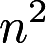
\includegraphics[width=0.16667in,height=0.15625in]{texmath/071fa15Cdpi7B3507Dn5E2}),在减少了比较次数方面它确实相当优秀,所以该算法仍然比直接插入排序好,故C选项错误且D选项正确。
\end{solution}
\question 对同一待排序序列分别进行折半插入排序和直接插入排序,两者之间可能的不同之处是(
)
\par\twoch{排序的总趟数}{元素的移动次数}{使用辅助空间的数量}{\textcolor{red}{元素之间的比较次数}}
\begin{solution}折半插入排序和直接插入排序相比主要是在有序区采用折半查找插入元素位置,当排序元素个数较多时会减少元素之间的比较次数,但不会减少元素的移动次数,也不会减少排序的总趟数。
【总结】如果考生一时想不出,也可以用简单的排序例子来进行解答。
\end{solution}
